\documentclass{article}

\usepackage[utf8]{inputenc}     % pdfLaTeX
\usepackage[T1]{fontenc}

\usepackage{amsmath, amsthm, amssymb}

\usepackage{tikz}
\usetikzlibrary{angles, quotes}


\title{Basic Geometry}
\author{Robin Rovenszky}
\date{Last updated: March 11, 2026}

\newtheorem{theorem}{Theorem}

\begin{document}

\maketitle
\tableofcontents
\newpage

\section{Theorems}

\begin{theorem}[Pythagorean Theorem]
In a right triangle with legs of lengths $a$ and $b$, and hypotenuse of length $c$, the following relation holds:
\[
a^2 + b^2 = c^2.
\]
\end{theorem}

\begin{proof}
Consider a square with side length $(a+b)$. Inside the square, place four identical right triangles with legs $a$ and $b$ and hypotenuse $c$, arranged so that their hypotenuses form a smaller square in the center.

The area of the large square is
\[
(a+b)^2.
\]

This area is also equal to the sum of the areas of the four triangles and the small central square.

Each triangle has area
\[
\frac{1}{2}ab,
\]
so the four triangles together have area
\[
4 \cdot \frac{1}{2}ab = 2ab.
\]

The remaining central square has side length $c$, so its area is
\[
c^2.
\]

Thus,
\[
(a+b)^2 = 2ab + c^2.
\]

Expanding the left-hand side gives
\[
a^2 + 2ab + b^2 = 2ab + c^2.
\]

Subtracting $2ab$ from both sides yields
\[
a^2 + b^2 = c^2.
\]

This proves the theorem.
\end{proof}


\begin{theorem}[Thales' Theorem]
Let $A$, $B$, and $C$ be points on a circle such that $AC$ is a diameter. 
Then $\angle ABC = 90^\circ$.
\end{theorem}

\begin{center}
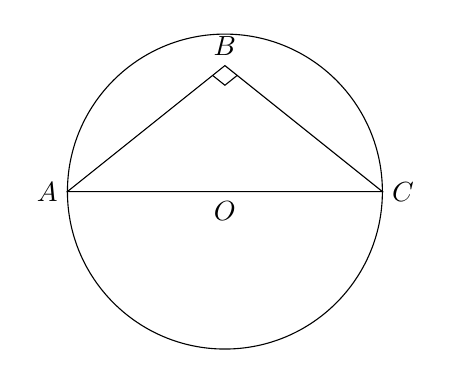
\begin{tikzpicture}[scale=2]

% Points
\coordinate (A) at (-1,0);
\coordinate (C) at (1,0);
\coordinate (B) at (0,0.8);
\coordinate (O) at (0,0);

% Circle
\draw (O) circle (1);

% Triangle
\draw (A) -- (B) -- (C) -- cycle;

% Diameter
\draw[dashed] (A) -- (C);

% Labels
\node[left] at (A) {$A$};
\node[right] at (C) {$C$};
\node[above] at (B) {$B$};
\node[below] at (O) {$O$};

% Right angle mark
\pic [draw, angle radius=0.2cm] {right angle = A--B--C};

\end{tikzpicture}
\end{center}

\begin{proof}
Let $O$ be the center of the circle. Since $AC$ is a diameter, $O$ is the midpoint of $AC$.

Because $OA = OB = OC$ (radii of the circle), triangles $OAB$ and $OCB$ are isosceles. 
Thus,
\[
\angle OAB = \angle OBA \quad \text{and} \quad \angle OCB = \angle OBC.
\]

Now consider triangle $ABC$. The angle at $B$ can be written as
\[
\angle ABC = \angle OBA + \angle OBC.
\]

Using the isosceles triangle relations:
\[
\angle OBA = \frac{180^\circ - \angle AOB}{2}, \quad
\angle OBC = \frac{180^\circ - \angle BOC}{2}.
\]

Since $A$, $O$, and $C$ are collinear, we have:
\[
\angle AOB + \angle BOC = 180^\circ.
\]

Therefore,
\[
\angle ABC 
= \frac{180^\circ - \angle AOB}{2} + \frac{180^\circ - \angle BOC}{2}
\]
\[
= \frac{360^\circ - (\angle AOB + \angle BOC)}{2}
= \frac{360^\circ - 180^\circ}{2}
= \boxed{90^\circ} \, .
\]

% TODO: Add kerületi és középponti szögek tétele, in Juhász maths notebook

Hence, $\angle ABC$ is a right angle.
\end{proof}

\newpage

\section{Related Problems}
\subsection{Problem 1.}

First Pythagorean Theorem:
\begin{equation}
    12^2 + x^2 = 15^2
\end{equation}
\begin{equation}
    144+x^2 = 225
\end{equation}
\begin{equation}
    x^2 = 81
\end{equation}
\begin{equation}
    x = 9
\end{equation}
Second Pythagorean Theorem:
\begin{equation}
    12^2 + y^2 = 13^2
\end{equation}
\begin{equation}
    144 + y^2 = 169
\end{equation}
\begin{equation}
    y^2 = 25
\end{equation}
\begin{equation}
    y = 5
\end{equation}
Thus our final answer is $x + y = 14$. \qed

\subsection{Problem 2.}

First Pythagorean Theorem:
\begin{equation}
    x^2 + (12-r)^2 = (12+r)^2
\end{equation}
Second Pythagorean Theorem:
\begin{equation}
    x^2 + r^2 = (24-r)^2
\end{equation}
Evaluating (9) - (10):
\begin{equation}
    (12-r)^2 - r^2 = (12+r)^2 - (24-r)^2
\end{equation}
\begin{equation}
    (12-2r) \cdot 12 = 36 \cdot (2r - 12)
\end{equation}
Dividing by 12 yields:
\begin{equation}
    (12-2r) = (2r - 12) \cdot 3
\end{equation}
Then dividing by 2:
\begin{equation}
    6-r = 3 \cdot (r-6)
\end{equation}
\begin{equation}
    6-r = 3r - 18
\end{equation}
Adding 18+r:
\begin{equation}
    24 = 4r
\end{equation}
\begin{equation}
    r = 6
\end{equation}
\qed

\subsection{Problem 3.}
\begin{theorem}[Theorem 1.]
For a parallelogram, we have
\begin{equation}
    e^2 + f^2 = a^2 \cdot2 + b^2 \cdot2
\end{equation}
\begin{proof}
First Pythagorean Theorem:
\begin{equation}
    (a-x)^2 + m^2 = e^2
\end{equation}
Second Pythagorean Theorem:
\begin{equation}
    (a+x)^2 + m^2 = f2
\end{equation}
Evaulating (19) + (20):
\begin{equation}
    a^2 - 2ax + x^2 + m^2 + a^2 + 2ax + x^2 + m^2 = e^2 + f^2
\end{equation}
Simplifying and invoking $m^2 + x^2 = b^2$:
\begin{equation}
    2a^2 + 2b^2 = e^2 + f^2
\end{equation}
\end{proof}

\end{theorem}

\subsection{Problem 4.}
Let the small circle's radius be $r$.\\
First Pythagorean Theorem:
\begin{equation}
    x^2 + (12 - r)^2 = (12 + r)^2
\end{equation}
Second Pythagorean Theorem:
\begin{equation}
    r^2 + x^2 = (24-r)^2
\end{equation}
See (1.2) Related Problems: Problem 2. for solution. These are two equivalent problems, under a 90 degree rotation. See figures for clarification.

\subsection{Problem 5.}
Let's put the circles inside rectangles instead of other circles!\\
We seek to find the height of the rectangle given the diameter of the small circles.\\
$r_0 = 12$

\subsection{Problem 6.}
Another circle-inside-rectangle problem. The rectangle is 60x48, what is the radius of the small circles?
\end{document}